%%%%%%%%%%%%%%%%%%%%%%%%%%%%%%
% COMBINATION OF INFORMATION %
%%%%%%%%%%%%%%%%%%%%%%%%%%%%%%
In the preceding \cref{sec:PEM:ProbInv} we declared the hyperparameters \(\bm{\theta}_{\bm{X}}\) as QoI and latent quantities \(\tuple{\bm{x}_i}\) as nuisance.
% OPTIMAL ESTIMATION
When this choice is reversed, i.e.\ proclaiming \(\tuple{\bm{x}_i}\) as the QoI and treating \(\bm{\theta}_{\bm{X}}\) as nuisance,
then the Bayesian multilevel model \cref{eq:PEM:ProbInv:Model} allows for an optimal type of inference \cite{Nagel:ICVRAM2014:Proc}.
% BORROWING STRENGTH
This effect is sometimes referred to as \textit{optimal combination of information} or \textit{borrowing strength}.
To our best knowledge, it has been pointed out for the first time in \cite{Multilevel:Draper1992}.
% OPTIMALITY
As we will see, the term ``optimal'' has to be understood with respect to the total amount of information processed, e.g.\ the acquired data and the available parametric and structural prior knowledge.
% STRONG STATEMENT
Optimal combination of information seems to be largely understudied in inverse problems with missing data structure.
By taking the marginal viewpoint of \cref{eq:PEM:ProbInv:MarginalPosterior}, the additional advantages that the joint formulation \cref{eq:PEM:ProbInv:JointPosterior} offers are often overlooked.
\par % ONE SPECIFIC
Based on the hierarchical model \cref{eq:PEM:ProbInv:Model}, in this section we will show how to ``borrow strength'' in inverse problems.
The optimal inference of a specific \(\bm{x}_{\analyzed}\) for some \(\analyzed \in \{1,\ldots,n\}\) is demonstrated.
We pursue three different estimation programs in order to investigate how inferring \(\bm{x}_{\analyzed}\) can be accomplished by wholly or only partially utilizing the informational resources.
% SECTION OUTLINE
In \cref{sec:PEM:CombInf:SimpleUpdating} we will present a simple Bayesian updating approach,
in respect to which the principle and mechanism of borrowing strength is emphasized by means of multilevel inference in \cref{sec:PEM:CombInf:MultilevelAnalysis}.
Beforehand we will devise a sequential filtering approach in \cref{sec:PEM:CombInf:SequentialFiltering} that will serve as an illustration of the underlying flow of information.

\subsection{Simple updating} \label{sec:PEM:CombInf:SimpleUpdating}
% INFORMATION
In this first approach, inference of \(\bm{x}_{\analyzed}\) will be solely based on the single observation \(\bm{y}_{\analyzed}\),
the informational content of \(f_{\bm{E}} (\bm{y}_{\analyzed}-\mathcal{M}(\bm{x}_{\analyzed},\bm{d}_{\analyzed}) \distparam \bm{\Sigma}_{\analyzed})\),
the structural prior \(f_{\bm{X} \cond \bm{\Theta}_{\bm{X}}} (\bm{x}_{\analyzed} \cond \bm{\theta}_{\bm{X}})\) and the parametric prior \(\pi_{\bm{\Theta}_{\bm{X}}} (\bm{\theta}_{\bm{X}})\).
% SIMPLE PRIOR
Utilizing the prior information one can formulate a Bayesian prior distribution for \(\bm{x}_{\analyzed}\).
By marginalizing over the hyperparameters \(\bm{\theta}_{\bm{X}}\) this reads as
\begin{equation} \label{eq:PEM:CombInf:SimpleUpdating:Prior}
  \pi(\bm{x}_{\analyzed}) = \int\limits_{\mathcal{D}_{\bm{\theta}_{\bm{X}}}}
  f_{\bm{X} \cond \bm{\Theta}_{\bm{X}}} (\bm{x}_{\analyzed} \cond \bm{\theta}_{\bm{X}}) \, \pi_{\bm{\Theta}_{\bm{X}}}(\bm{\theta}_{\bm{X}}) \, \mathrm{d} \bm{\theta}_{\bm{X}}.
\end{equation}
This compound distribution represents the uncertainty that \(\bm{x}_{\analyzed}\) priorly carries.
% SIMPLE POSTERIOR
Ensuing from the prior \cref{eq:PEM:CombInf:SimpleUpdating:Prior}, analyzing the piece of data \(\bm{y}_{\analyzed}\) is accomplished by constructing the corresponding posterior.
It is proportional to \(\pi(\bm{x}_{\analyzed} \cond \bm{y}_{\analyzed}) \propto f_{\bm{E}} ( \bm{y}_{\analyzed}-\mathcal{M}(\bm{x}_{\analyzed},\bm{d}_{\analyzed}) \distparam \bm{\Sigma}_{\analyzed} ) \, \pi(\bm{x}_{\analyzed})\).
% HIERARCHICAL BAYES
We remark that the approach is formally reminiscent of hierarchical inversion as discussed in \cref{sec:PEM:ProbInv}.
\par % INFORMATION
While the observation \(\bm{y}_{\analyzed}\) that is directly associated to \(\bm{x}_{\analyzed}\) has been analyzed,
the evidence that \(\tuple{\bm{y}_{\notanalyzed}}\) carry about \(\bm{\theta}_{\bm{X}}\), and in turn about \(\bm{x}_{\analyzed}\), has not yet been taken into consideration.
Put another way, the hierarchical problem structure has been respected by formulating \cref{eq:PEM:CombInf:SimpleUpdating:Prior}, however, it has only been partially exploited for learning about the QoI \(\bm{x}_{\analyzed}\).

\subsection{Sequential filtering} \label{sec:PEM:CombInf:SequentialFiltering}
% NOTATION
For the second estimation scheme, which will be based on sequential updating,
we introduce the simplifying notation \(\tuple{\bm{q}_{\notanalyzed}} = (\bm{q}_1,\ldots,\bm{q}_{\analyzed-1},\bm{q}_{\analyzed+1},\ldots,\bm{q}_n)\).
% FILTERING PRIOR
In a first step probabilistic inversion is accomplished by estimating \(\bm{\theta}_{\bm{X}}\) with the data \(\tuple{\bm{y}_{\notanalyzed}}\).
Similarly to \cref{eq:PEM:CombInf:SimpleUpdating:Prior}, the resulting posterior \(\pi(\bm{\theta}_{\bm{X}} \cond \tuple{\bm{y}_{\notanalyzed}})\) can be translated into a mixture distribution
\begin{equation} \label{eq:PEM:CombInf:SequentialFiltering:Prior}
  \pi \big( \bm{x}_{\analyzed} \cond \tuple{\bm{y}_{\notanalyzed}} \big) = \int\limits_{\mathcal{D}_{\bm{\theta}_{\bm{X}}}}
  f_{\bm{X} \cond \bm{\Theta}_{\bm{X}}} (\bm{x}_{\analyzed} \cond \bm{\theta}_{\bm{X}}) \, \pi \big( \bm{\theta}_{\bm{X}} \cond \tuple{\bm{y}_{\notanalyzed}} \big) \, \mathrm{d} \bm{\theta}_{\bm{X}}.
\end{equation}
It represents the uncertainty in \(\bm{x}_{\analyzed}\) following the analysis of \(\tuple{\bm{y}_{\notanalyzed}}\) but prior to analyzing \(\bm{y}_{\analyzed}\).
Thereupon the second stage of the filtering program consists in utilizing \cref{eq:PEM:CombInf:SequentialFiltering:Prior} as a Bayesian prior for inferring \(\bm{x}_{\analyzed}\) by inverting \(\bm{y}_{\analyzed}\).
% FILTERING POSTERIOR
Bayesian updating yields the posterior distribution \(\pi(\bm{x}_{\analyzed} \cond \tuple{\bm{y}_{\notanalyzed}},\bm{y}_{\analyzed})
\propto f_{\bm{E}} (\bm{y}_{\analyzed}-\mathcal{M}(\bm{x}_{\analyzed},\bm{d}_{\analyzed}) \distparam \bm{\Sigma}_{\analyzed}) \, \pi(\bm{x}_{\analyzed} \cond \tuple{\bm{y}_{\notanalyzed}})\).
\par % INFORMATION
Information-wise, the estimation of \(\bm{\theta}_{\bm{X}}\) has been initially based on the data \(\tuple{\bm{y}_{\notanalyzed}}\),
its conditional distributions \(f_{\bm{E}} (\bm{y}_i-\mathcal{M}(\bm{x}_i,\bm{d}_i) \distparam \bm{\Sigma}_i)\) for \(i \neq \analyzed\),
the structural knowledge \(f_{\bm{X} \cond \bm{\Theta}_{\bm{X}}} (\bm{x}_i \cond \bm{\theta}_{\bm{X}})\) and the parametric prior \(\pi_{\bm{\Theta}_{\bm{X}}} (\bm{\theta}_{\bm{X}})\).
While inheriting the obtained information about \(\bm{\theta}_{\bm{X}}\) by means of \cref{eq:PEM:CombInf:SequentialFiltering:Prior},
the observation \(\bm{y}_{\analyzed}\) has been eventually inverted for \(\bm{x}_{\analyzed}\).

\subsection{Multilevel inversion} \label{sec:PEM:CombInf:MultilevelAnalysis}
% JOINT & MARGINAL POSTERIOR
A full hierarchical analysis constitutes the third type of estimation.
By formulating the joint posterior \cref{eq:PEM:ProbInv:JointPosterior} of the collectivity of unknowns \((\tuple{\bm{x}_i},\bm{\theta}_{\bm{X}})\)
and marginalizing over nuisance \((\tuple{\bm{x}_{\notanalyzed}},\bm{\theta}_{\bm{X}})\), the posterior distribution of the QoI \(\bm{x}_{\analyzed}\) can be written as
\begin{equation} \label{eq:PEM:CombInf:MultilevelAnalysis:Posterior}
  \pi \big( \bm{x}_{\analyzed} \cond \tuple{\bm{y}_i} \big) = \int\limits_{\mathcal{D}_{\bm{x}}^{n-1}} \int\limits_{\mathcal{D}_{\bm{\theta}_{\bm{X}}}}
  \pi \big( \tuple{\bm{x}_i},\bm{\theta}_{\bm{X}} \cond \tuple{\bm{y}_i} \big) \, \mathrm{d} \tuple{\bm{x}_{\notanalyzed}} \, \mathrm{d} \bm{\theta}_{\bm{X}},
\end{equation}
where \(\mathrm{d} \tuple{\bm{x}_{\notanalyzed}} = \mathrm{d}\bm{x}_1 \ldots \mathrm{d}\bm{x}_{\analyzed-1} \, \mathrm{d}\bm{x}_{\analyzed+1} \ldots \mathrm{d}\bm{x}_n\).
% JOINT POSTERIOR SAMPLING
Note that when the joint posterior \cref{eq:PEM:ProbInv:JointPosterior} is computed, other marginals than \cref{eq:PEM:CombInf:MultilevelAnalysis:Posterior} can be extracted similarly.
\par % INFORMATION
In terms of estimating \(\bm{x}_{\analyzed}\), the structure of the posterior \cref{eq:PEM:CombInf:MultilevelAnalysis:Posterior} reveals that
all the different pieces of information have been ``optimally'' combined during a joint learning process.
From an informational point of view, the total data \(\tuple{\bm{y}_i}\), their conditional distributions \(f_{\bm{E}} (\bm{y}_i-\mathcal{M}(\bm{x}_i,\bm{d}_i) \distparam \bm{\Sigma}_i)\),
the structural knowledge \(f_{\bm{X} \cond \bm{\Theta}_{\bm{X}}} (\bm{x}_i \cond \bm{\theta}_{\bm{X}})\) and the hyperprior \(\pi_{\bm{\Theta}_{\bm{X}}} (\bm{\theta}_{\bm{X}})\) have been completely synthesized.
This implies that inferring \(\bm{x}_{\analyzed}\) ``borrows'' information encoded in the observations \(\tuple{\bm{y}_{\notanalyzed}}\).
% FLOW OF INFORMATION
A DAG-based visualization of the underlying flow of information is provided in \cref{fig:PEM:DAG:CombInf}.
% EXCHANGEABILITY
The deeper reason for borrowing strength to happen is the partial reducibility of the uncertainty model \cref{eq:PEM:Multilevel:Exchangeability}, i.e.\ the exchangeability of aleatory variables \(\tuple{\bm{x}_i}\).
% DAG
\begin{figure}[ht]
  \centering
  \includegraphics[height=4cm]{fig_PEM_DAG_CombinationInformation}
  \caption[Optimal combination of information]{Optimal combination of information.
           A Bayesian network representation of probabilistic inversion is shown.
           Known (\(\vcenter{\hbox{\protect\includegraphics[height=1.2ex]{fig_Square}}}\))
           and unknown (\(\vcenter{\hbox{\protect\includegraphics[height=1.3ex]{fig_Circle}}}\)) quantities
           are related by probabilistic (\(\vcenter{\hbox{\protect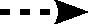
\includegraphics[height=1.0ex]{fig_Dashed}}}\)) relations.
           The ``upstream'' (\(\vcenter{\hbox{\protect
\includegraphics[height=1.0ex]{fig_Backward}}}\))
           and ``downstream'' (\(\vcenter{\hbox{\protect
\includegraphics[height=1.0ex]{fig_Forward}}}\))
           flow of information towards a specific \(\bm{x}_{\analyzed}\) is indicated.
           This is a form of borrowing strength.
          }
  \label{fig:PEM:DAG:CombInf}
\end{figure}